\documentclass[11pt, oneside]{article} 
\usepackage{geometry}
\geometry{letterpaper} 
\usepackage{graphicx}
	
\usepackage{amssymb}
\usepackage{amsmath}
\usepackage{parskip}
\usepackage{color}
\usepackage{hyperref}

\graphicspath{{/Users/telliott_admin/Tex/png/}}
% \begin{center} 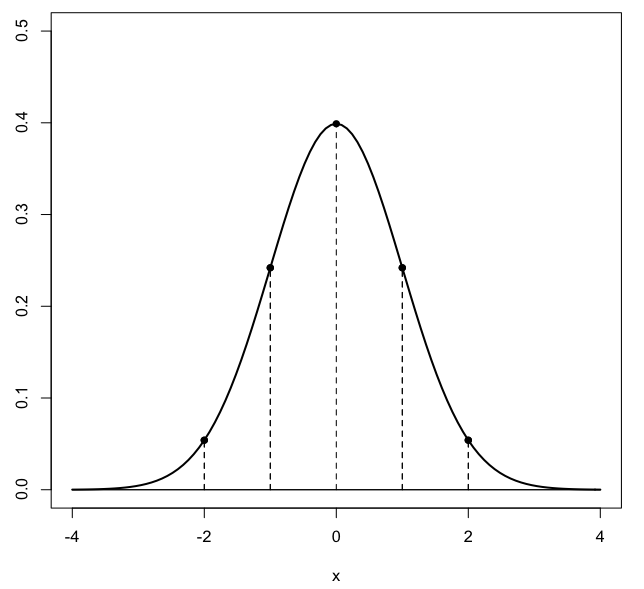
\includegraphics [scale=0.4] {gauss3.png} \end{center}

\title{Apple core}
\date{}

\begin{document}
\maketitle
\Large
\begin{center} 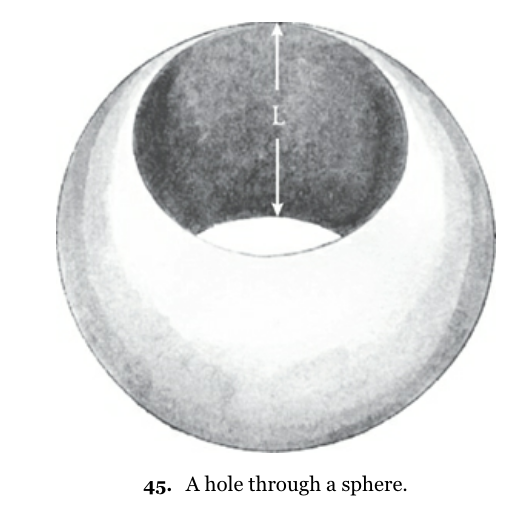
\includegraphics [scale=0.4] {knapkin_ring.png} \end{center}

Another great problem I want to explore is the shape sometimes called "the cored apple" (Adams et al.) but it is probably more famous as the "napkin ring" problem.

\url{https://en.wikipedia.org/wiki/Napkin_ring_problem}

The figure from Acheson, above, is telling.  It gives only one length, and that is $L$, the depth of the hole.  The reason is that the volume of the remaining solid is \emph{independent of the size of the sphere}.  That's pretty amazing.  In fact
\[ V = \frac{\pi}{6} L^3 \]

\subsection*{fast solution}
Recall from the chapter on the spherical cap that we can get the volume of the sphere by integrating slices perpendicular to an axis, say the $x$-axis.  The slices are circles with radius $r$ where

\begin{center} 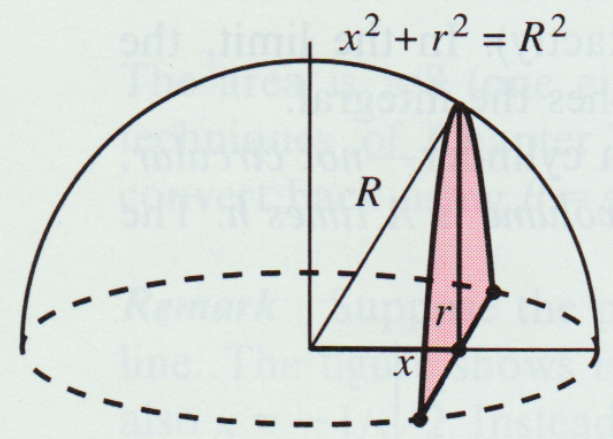
\includegraphics [scale=0.3] {sph_slices2.png} \end{center}
\[ r^2 + x^2 = R^2 \]
and the area of each slice is
\[ A = \pi r^2 = \pi \ [ \ R^2 - x^2 \ ] \]
The volume is just the integral
\[ V = \int_{-R}^{R} \pi \ [ \ R^2 - x^2 \ ] \ dx \] 
Since this is an even function, we can start from $0$ and multiply by $2$:
\[ V = 2 \int_{0}^{R} \pi \ [ \ R^2 - x^2 \ ] \ dx \] 
The integral is easy
\[ V = 2 \pi \ [ \ R^2 x - \frac{x^3}{3} \ ] \ \bigg |_0^R \]

What is great about this is that we can get the partial volume by integrating to any height.  While we could use $L/2$ for this height, it simplifies the arithmetic to set
\[ H = \frac{L}{2} \]

The area of the sphere minus the caps (but including the central cylinder) is
\[ V = 2 \pi \ [ \ R^2 x - \frac{x^3}{3} \ ] \ \bigg |_0^{H} \]
\[ = 2 \pi \ [ \ R^2H - \frac{1}{3} \ H^3 \ ] \]

All we need now is to find the area of the cylinder.  

We are given $H$.  We need the radius $r$ but (referring back to the previous figure) we know that
\[ R^2 = H^2 + r^2 \]
so the area of the base of the cylinder is
\[ A = \pi r^2 = \pi \ [ \ R^2 - H^2 \ ] \]

and the volume of the cylinder is
\[ V = 2H \cdot \pi \ [ \ R^2 - H^2 \ ] \]
Bringing the $H$ inside, we obtain:
\[ V = 2 \pi \ [ \ HR^2 - H^3 \ ] \]

The volume we seek is the volume of the sphere minus its caps, minus the area of the cylinder.
\[ V = 2 \pi \ [ \ R^2H - \frac{1}{3} \ H^3 - HR^2 + H^3 \ ] \]
The magic is that the terms with $R^2$ cancel so we have
\[ V = 2 \pi \ [ \ - \frac{1}{3} \ H^3  + H^3 \ ] \]
\[ = \frac{4}{3} \pi \ H^3 \]
\[ = \frac{\pi}{6} \ L^3 \]

\subsection*{geometry}
\begin{center} 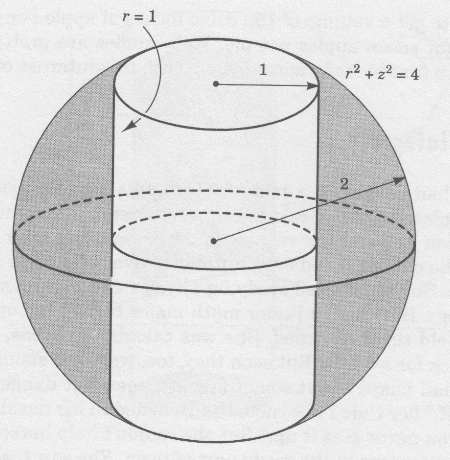
\includegraphics [scale=0.3] {apple_core.png}  \end{center}
In Adams we are given the same problem but we don't have $L$, rather the radius of the sphere and the inset cylinder are given instead.

A sphere of radius $2$ has had the central portion consisting of a cylinder plus the two spherical caps removed.

We are given that the cylinder has radius $1$.  The height $L$ is an unknown.

Recall that 
\[ R^2 = (\frac{L}{2})^2 + r^2 \]
So
\[ 3 = (\frac{L}{2})^2 \]
\[ L = 2 \sqrt{3} \]

Hence, substituting into the formula from the above analysis
\[ V = \frac{\pi}{6} \ (2 \sqrt{3})^3 = \pi \ \frac{8 \cdot 3 \cdot \sqrt{3}}{6} \]
\[ = 4 \sqrt{3} \pi \]

Another way to do this problem is to find the volume of each spherical cap.  We worked this out in the previous chapter.  
\begin{center} 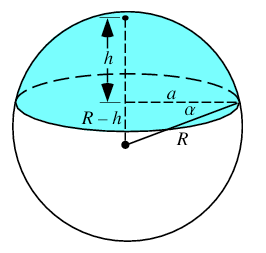
\includegraphics [scale=0.6] {spherical_cap.png} \end{center}

We use $h$ here for the height instead of $L$.  If $h$ is the height of the cap, then its volume is
\[ V_{cap} = \frac{1}{3} \pi h^2(3R - h) \]

We are given the radius of the core, which is labeled $a$ in the second figure.  The equation we get using the Pythagorean theorem is
\[ (R - h)^2 + a^2 = R^2  \]
\[ R^2 - 2Rh + h^2 + a^2 = R^2 \]
We know that $R=2$ and $a=1$ so this simplifies to
\[ h^2 - 4h + 1 = 0 \]
Solve this using the quadratic formula to obtain:
\[ h = 2 \pm \ \sqrt{3} \]
Since $h$ cannot be greater than $R$ we take the negative square root:
\[ h = 2 - \sqrt{3} \]
\[ h^2 = 7 - 4 \sqrt{3} \]
We confirm that this value of $h$ solves the quadratic equation.

The volume of one spherical cap is
\[ V_{cap} = \frac{1}{3} \pi h^2(3R - h) \]
So 
\[ h^2(3R - h) = (7- 4 \sqrt{3})(6-(2-\sqrt{3})) \]
\[ = (7- 4 \sqrt{3})(4 + \sqrt{3})) \]
\[ = 28 - 12 + (-16 + 7) \sqrt{3} \]
\[ = 16 - 9 \sqrt{3} \]

We have two of these
\[ V = 2 \cdot \frac{\pi}{3} \cdot (16 - 9 \sqrt{3}) \]

The volume of the cylinder is the area of the cross-section
\[ \pi \cdot 1^2 = \pi \]
 times the height, which is $2(R-h) = 2 \sqrt{3}$.
\[ V = 2 \pi \sqrt{3} \]
We have to subtract both of these from the volume of the whole sphere, which is $32 \pi/3$.  The desired quantity is
\[ V = \frac{32 \pi}{3} - 2 \pi \sqrt{3} - \frac{2\pi}{3} \ (16 - 9 \sqrt{3}) \]
\[ = \pi \ [ \ \frac{32}{3} - 2 \sqrt{3} - \frac{2}{3} \ (16 - 9 \sqrt{3}) \ ] \]
\[ = \pi \ [ \ - 2 \sqrt{3} - \frac{2}{3} \ ( - 9 \sqrt{3}) \ ] \]
\[ = \pi \ [ \ 4 \sqrt{3}) \ ] \]

\subsection*{calculus}

There are several more elegant approaches from calculus.  

Consider the sphere as a surface above the circle.  For the circle we have $x^2 + y^2 = r^2$, where now we are using $r$ as a \emph{variable} that could range from $0 \rightarrow R$.

In Cartesian coordinates the circle is
\[ x^2 + y^2 + z^2 = R^2 \]
Using polar coordinates for $x$ and $y$ we have 
\[ r^2 + z^2 = R^2 \]
\[ z = \sqrt{R^2 - r^2} = \sqrt{4 - r^2}  \]
We will do a double integral over the the $xy$-plane, adding up the value of this function for each small area element $dA$.  In polar coordinates, the area element is
\[ dA = r \ dr \ d \theta \]
so, for example, the basic area integral is
\[ A = \int dA = \int_{\theta=0}^{2 \pi} \int_{r=0}^R r \ dr \ d \theta = \int_{\theta=0}^{2 \pi} \frac{1}{2}R^2 \ d \theta = \pi R^2 \]

Now, what we want is to integrate the surface height over the whole area, plugging in from above we get
\[ V = \int dV = \int_{\theta=0}^{2 \pi} \int_{r=0}^R \sqrt{R^2 - r^2}  \ r \ dr \ d \theta \]
This integral is not hard to do because we have the derivative of what is under the square root sign.  Let $u = R^2 - r^2$.  Then
\[ du = -2r \ dr \]
\[ -\frac{1}{2} \ du = r dr \]
so the inner integral is
\[ \int -\frac{1}{2} \sqrt{u} \  du = -\frac{1}{3} u^{3/2} \]
Substituting back, the inner integral (for the whole sphere) is 
\[ -\frac{1}{3} (R^2 -r^2)^{3/2} \bigg{|}_0^R = \frac{1}{3}(R^2)^{3/2} =  \frac{1}{3} R^3 \]

When we do the outer integral we pick up an extra factor of $2\pi$, which gives the correct value for the volume of the hemisphere.
What is great about this approach is that we don't have to start at $r=0$.  This simplifies our problem enormously.  In the problem, we start from $r=1$ (and we have $R=2$).  So this gives the volume we seek as
\[ V = \int dV = \int_{\theta=0}^{2 \pi} \int_{r=1}^2 \sqrt{4 - r^2}  \ r dr d \theta \]
The inner integral is
\[ -\frac{1}{3} (4 -r^2)^{3/2} \bigg{|}_1^2 = \frac{1}{3}(3)^{3/2} =  \sqrt{3} \]
Now we have
\[ V =  \int_{\theta=0}^{2 \pi} \sqrt{3} \ d \theta \]
which is just $2\pi \sqrt{3}$.  Multiply by $2$ for the whole apple, we get $4 \pi \sqrt{3}$.  This matches what we had previously.

\subsection*{rings}
Consider a sphere of radius $R$ and a bored hole of radius $a$.  The height of the cylinder (and the part of the sphere that remains) is 
\[ H^2 = R^2 - a^2 \]

Take horizontal cross-sections.  For each one, we get a ring (a plane annulus).  The area of a cross-section depends on the difference between the outer and the inner rings.  The inner ring is constant ($a^2$) and the outer ring depends on the height above the $x,y$-plane, $h$.
\[ \text{outer}^2 = R^2 - h^2 \]
The difference is
\[ R^2 - h^2 - a^2 = H^2 - h^2 \]

If we were working before calculus, at this point we would notice that this is the difference between a cylinder of radius $H$ and a cone of variable height $h$, and use Cavalieri's principle.  Does this sound familiar?  Look back at Chapter 2 if it does not.

Instead, we let $h$ range from $[0,H]$
\[ V = 2 \int_0^H \pi (H^2 - h^2) \ dh \]
The factor of $2$ is to include the bottom hemisphere.
\[ = 2 \pi \ [ \ H^2 h - \frac{h^3}{3} \ ] \ \bigg |_0^H \]
\[ = \frac{4}{3} \pi H^3 \]

The result does not depend on $R$, only $H$.  (However, I don't find this so impressive, since if we specify the problem in terms of the radius $a$, then $R$ comes in).  Also, when $H = R$, we get the correct volume for the whole sphere.

The great advantage of calculus is that we could let the bounds on $h$ be any values in $[0,H]$.

In the previous problem, we had $R = 2$, $a = 1$ and so $H = \sqrt{3}$.  We obtain
\[ H^3 = 3 \sqrt{3} \]
\[ \frac{4}{3} \pi H^3 = 4 \pi \sqrt{3}  \]
which matches our previous result.

\subsection*{cylinders}
Or, use the method of cylinders.  Let $r$ range over $[a,R]$.  

For each $r$ we have a cylinder of circumference $2 \pi r$ and height $h = 2\sqrt{R^2 - r^2}$.  

The volume is
\[ \int_a^R 2 \pi r \  2\sqrt{R^2 - r^2} \ dr \]
\[ = 4 \pi \ [ \ \int_a^R \sqrt{R^2 - r^2} \ r \ dr \ ] \]
We already did this integral in a previous section.  The result is
\[ = -\frac{4}{3} \pi \ [ \ (R^2 - r^2)^{3/2} \ ] \bigg |_a^R  \]
\[ = \frac{4}{3} \pi \ [ \ (R^2 - a^2)^{3/2} \ ]  \]
\[ = \frac{4}{3} \pi \ [ \ (H^2)^{3/2} \ ]  \]
\[ = \frac{4}{3} \pi H^3 \]
Again.

\end{document}